% Author        : PokMan Ho pok.ho19@imperial.ac.uk
% Script        : predationModel.tex
% Desc          : three players predation model
% Input         : none
% Output        : pdf report in same directory
% Arguments     : 0
% Date          : Feb 2020

\documentclass[a4paper,11pt]{article}
\usepackage[margin=2cm]{geometry}
\usepackage[english]{babel}
\usepackage{graphicx, longtable, amsmath, amssymb, csquotes}
\graphicspath{{graph/}{graph/}}

\usepackage{xcolor,colortbl}
\definecolor{green}{rgb}{0,.4,0}

\usepackage{hyperref}
\hypersetup{
	colorlinks=true,
	linkcolor=green,
	filecolor=red,      
	urlcolor=blue,
	citecolor=orange
}

%% citation
\usepackage[%
autocite 	= superscript,
backend 	= bibtex,
sortcites 	= true,
style 		= nature
]{biblatex}
\bibliography{predationModel.bib}

\newcommand{\ec}{\textit{E. coli}}
\newcommand{\am}{Amoeba}
\newcommand{\ap}{\textit{A. platensis} (Spirulina)}

\title{Predation in Eco-Bioelectric Cell}
\author{PokMan Ho}
\date{08 Feb 2020}

\begin{document}
    \maketitle
    \tableofcontents

    \section{Model in diagram}
    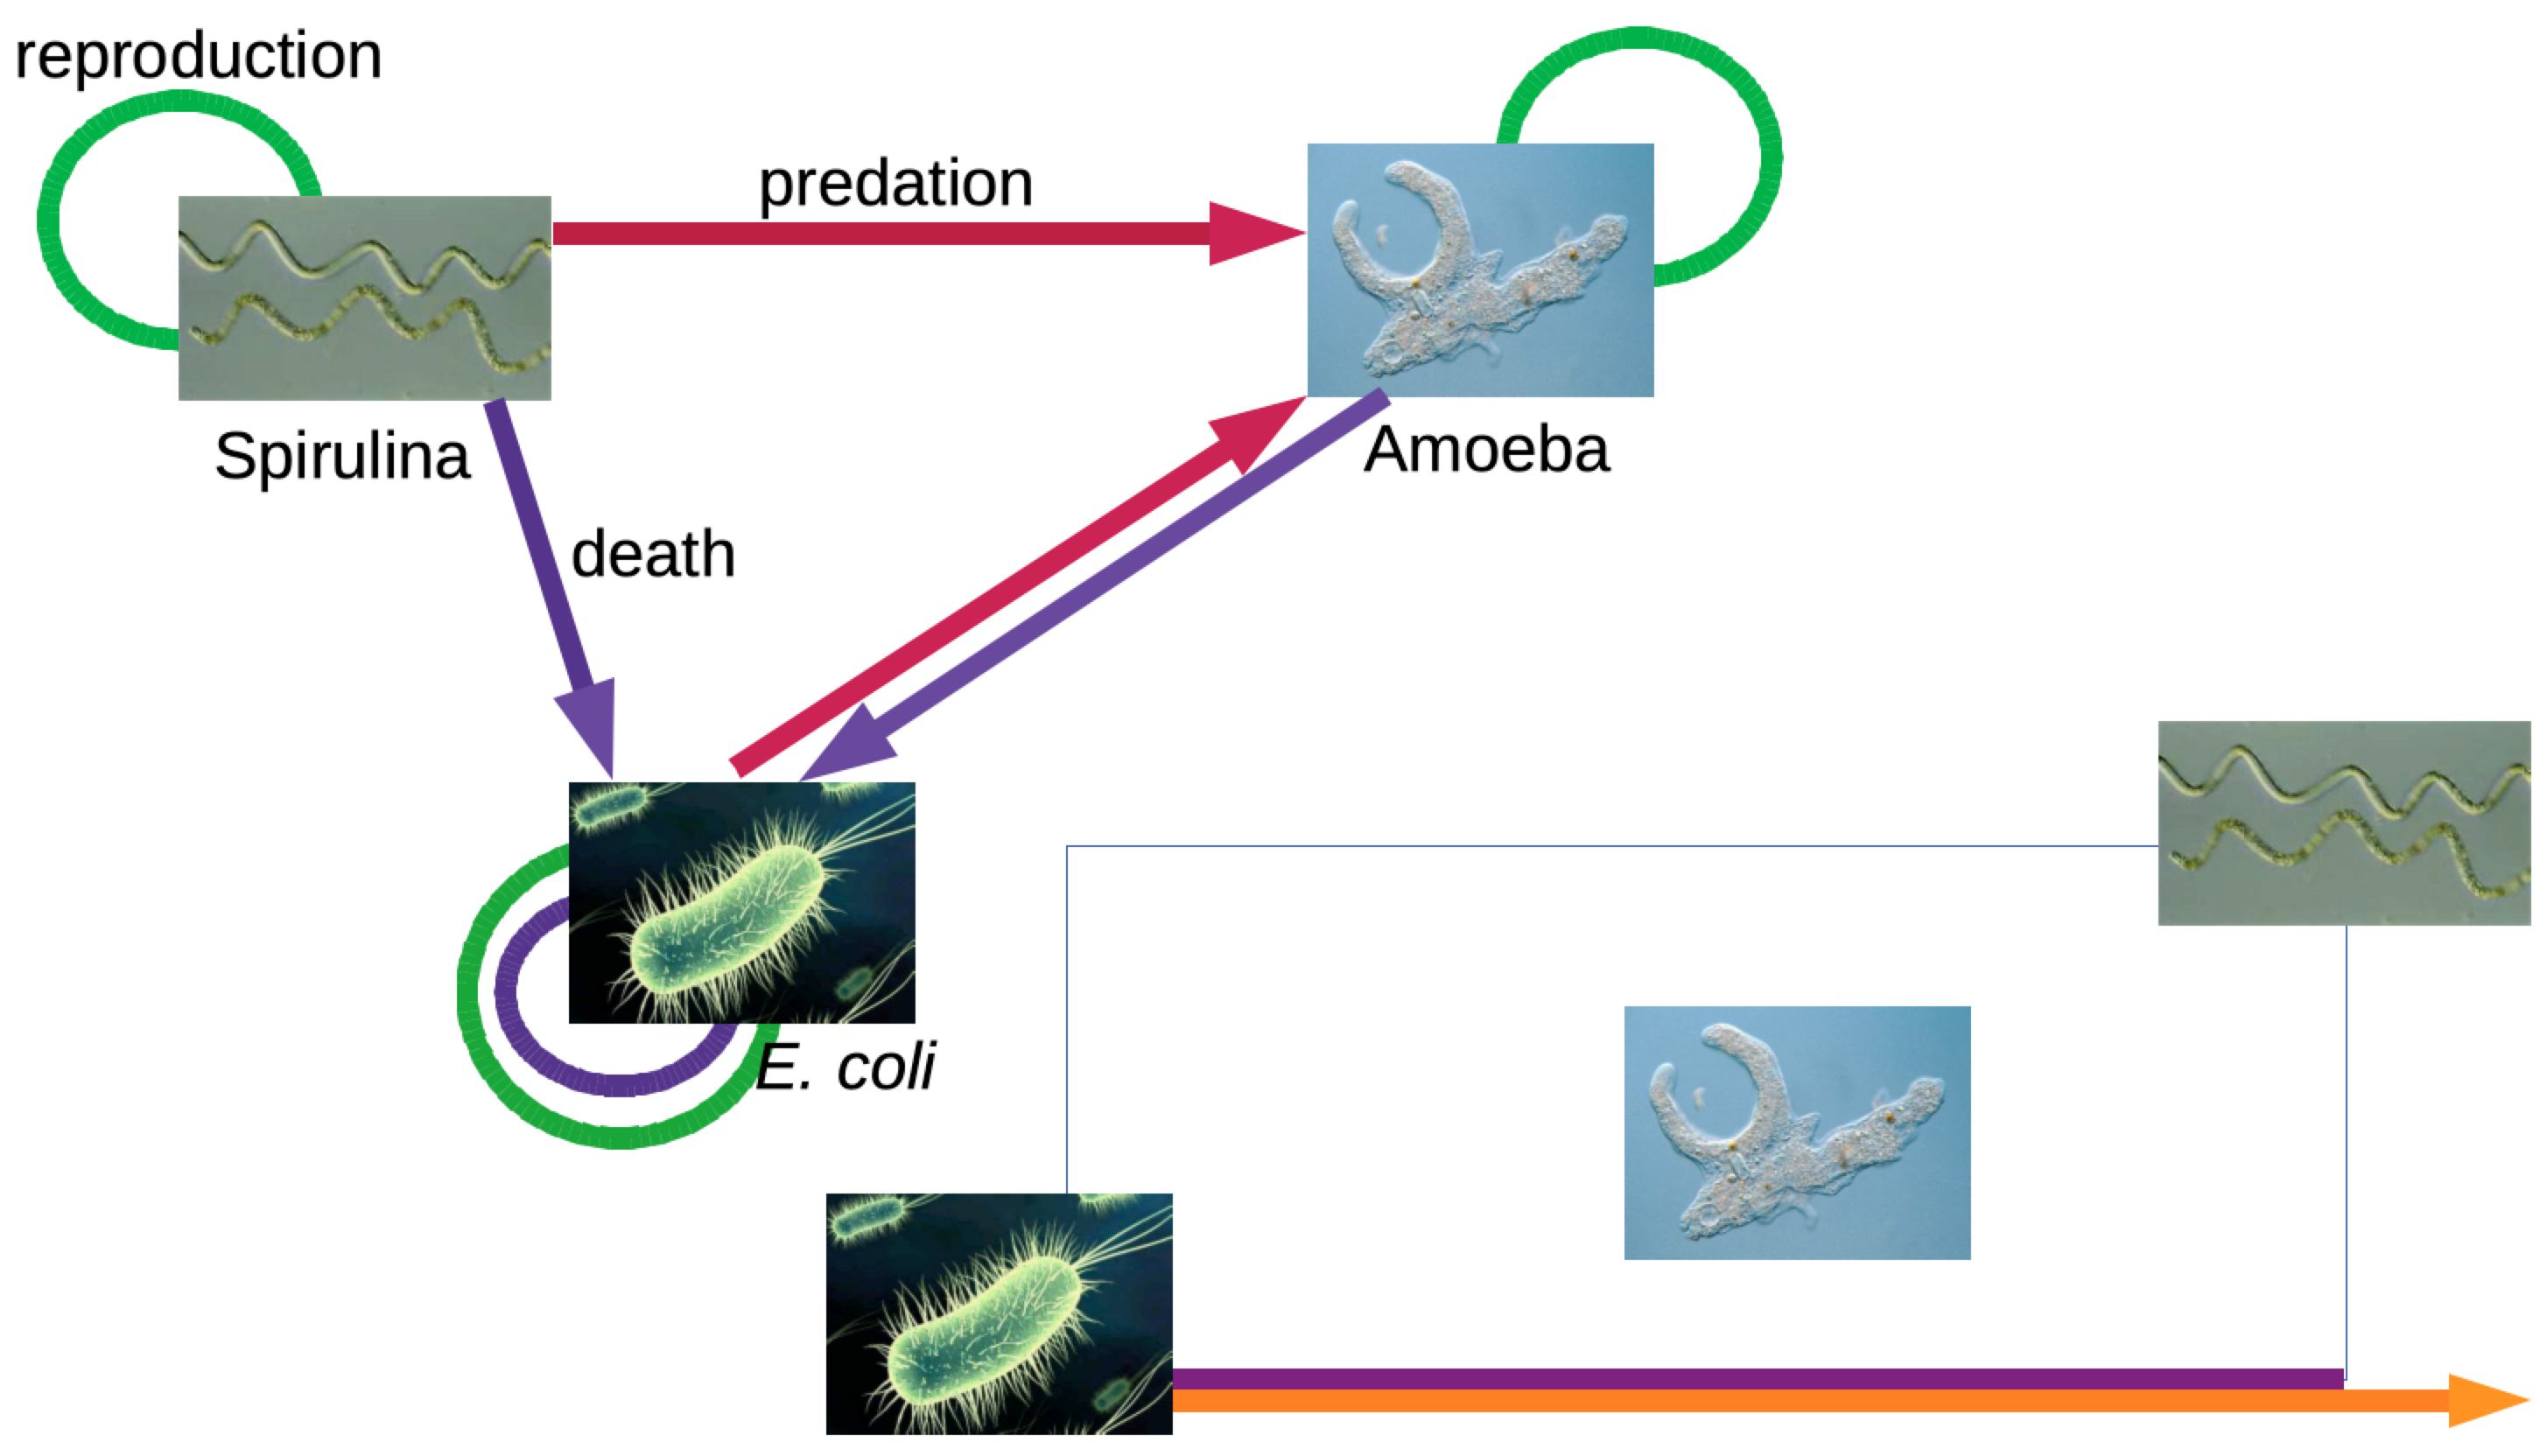
\includegraphics[width=\linewidth]{sandbox/graph/model.png}
    
    \section{Main considerations}
    \begin{itemize}
        \item metabolic theory determines energy transferring mechanism between trophic levels (i.e. arrows)
        \item solar intensity affect energy budget of primary production, which determines interaction rate between groups
        \item \ap\ as producer, expected to live at top of meta-ecosystem
        \item \am\ as mobile predator, expected to move between meta-ecosystems and pelagic columns foraging for the other two components for food
        \item \ec\ as detritivores, expected to stick tight to anode of the eco-bioelectric half-cell because of attraction between cytochrome D (cytD) and anode (orange arrow at bottom)
    \end{itemize}
    
    \section{Interaction ODEs in words}
    \begin{enumerate}
        \item 
    \end{enumerate}
    
    \section{conclusion}
    
    \nocite{*}\printbibliography
\end{document}